\documentclass{sig-alternate-05-2015}


\begin{document}

% Copyright
\setcopyright{acmcopyright}

\title{Report for seminar: Topics in Data Mining}
\subtitle{[on study of the paper: Oliveira, Márcia, and João Gama. "A framework to monitor clusters evolution applied to economy and finance problems."]
}
\numberofauthors{1}
\author{
\alignauthor Zijian Zhang\\
        \affaddr{Subject area: Informatik}\\
        \affaddr{Matriculation number: 3184680}\\
        \email{zhangzijian0523@gmail.com}
}

\maketitle
\begin{abstract}
In this report a short summary about studying of paper \emph{A framework to monitor clusters evolution applied to economy and finance problems.}(MCEEF) is presented. At first are a couple of real world's problems evolved being mentioned by the MCEEF paper introduced. Then we go into the framework, which is described by the paper, to see how in the world is the framework been defined, what functionalities does it have or which types of data phenomenons could it describe. Then the result and performance of appliance of this framework are to be illustrated. At last shortages that still exist within the framework are discussed and according to the paper we could also mention some probable improvement on the framework.
\end{abstract}

\section{Researches review}
Cluster structure and clustering problems of a bundle of data are fascinating topics in studying properties of data analysis. Being discussed in \cite{JAIN:Clustering} and so on. static data cluster was deeply researched. However, considering the variation of data alone with the time goes by, it dosen't make seance that clusters already gotten always keep as-is. A cluster could birth, die, slit and attributes of (clusters of) data set could illustrate interesting properties. That's why the temporal attributes, a.k.a. transitions, were discussed at first in different aspects, such as generic patterns\cite{GANTI:datachar}\cite{BARTOLINI:panda}\cite{CHAWATHE:changedetection}, clusters\cite{SPILIOPOULOU:transition}\cite{FALKOWSKI:socialnet}\cite{YANG:spatiotemporal} or association rules\cite{BARON:monitorminingresults}\cite{BARON:webusagepattern}.

At the aspect of static data, frameworks such as FOCUS\cite{GANTI:datachar} and MH-DIFF\cite{CHAWATHE:changedetection} provided a formal way to describe the structural component and measure component by researching the clustering of data set. Those frameworks also inspired the research on the differences or deviations between two cluster sets, or those between clustering of two snapshots of data set. With the help of tree structures built in $t_i$ and $t_{i+1}$, distance of two models are described using a set of editing operations.

Further researches like PAM(Automated Pattern Monitor)\cite{BARON:webusagepattern} expand the method of detection of derivation by combining GRM(Generic Rule Model) and monitoring using threshold as two different phases. That figured out a clearer way to go deep into the monitoring of clusters' evolution.

Based on the result of studying of social networks, an event-based framework\cite{FALKOWSKI:socialnet}\cite{ASUR:event} for characterizing the evolution of interaction networks was produced. The social networks were considered as time fluctuating graphs. The temporal behavior was categorized in to several critical events, such as \emph{formation}, \emph{dissolution}, \emph{split} and \emph{merge} of clusters (communities), or \emph{join}, \emph{leave}, \emph{appearance} or \emph{disappearance} of individuals(entities).

Confronted data streams, data analyzer usually focus on unsupervised learning of the patterns attend in data. Naturally clustering should to be main direction of research proceeded\cite{AGGARWAL:diagnosis}\cite{AGGARWAL:framework}\cite{CHEN:change}\cite{OCALLAGHAN:highquality}\cite{ELNEKAVE}\cite{KALNIS:movingclusters}\cite{LI:entropy}. Also because of the efficiency and scalability of algorithms. A corresponded generic tool to understand, visualize and diagnose differences between evolving data streams were also developed. Within these approaches, the concept of velocity density estimation are suggested been split into both temporal and spatial velocity profiles. While temporal velocity profiles provide the variation of the density rate over a given section of time; the spatial velocity profile describes the movement of data in a feature space within a fixed time point. Furthermore the events of data points are expanded with \emph{coagulation}, \emph{dissolution} and \emph{shift}. Also this framework could be extended to high-dimensional data streams.

According to the writer of this paper, there were still two research works are closely related to theirs, thus MONIC framework\cite{SPILIOPOULOU:transition} and it's improved version MONIC+ framework\cite{SPILIOPOULOU:tracing}. While MONIC uses a data aging function to detect the evolution of clustering, MONIC+ is less generic and introduces proper heuristic to capture transitions between different clusterings, which is independent of the clusters discovery process. Although MONIC and it's improvement were published by a same author, they seems to use differentmetric to detect evolution and do not provide a visualize approach. While this paper the author provide an approach which improves his former work\cite{OLIVEIRA:bipartite} and uses the same way, i.e. weighted bipartite graphs, to monitor the variation of clustering. Thus according to the author, those four papers are mutually substantive.

\section{Short description of MEC Framework}
To proceed the research on evolution of clusters. The essay at first provides two critical point about it: definition of clustering and the concept of temporal evolution. Our main interested part is definition and recognition of specific patterns of behaviour of clusters within time interval $[t_i, t_{i+\Delta t}] (\Delta t = 1,...,T-i)$.
\subsection{Definition of clusters and clustering}
The clusters, or a clustering of a set of data, is denoted as $\upsilon$ is a specific partitioning of a data set D into K partitions $\upsilon = {C_1,...,C_i,...C_k}$ and have three main properties:

    1.clusters should be \emph{disjoint}(or mutually exclusive)
        \begin{displaymath}
          C_i\cap C_j = \emptyset, \forall i\ne j
        \end{displaymath}

    2.clusters should be \emph{collectively exhausted}
        \begin{displaymath}
          \cup^K_{i=1}C_i=D
        \end{displaymath}

    3.Data points, or according to the essay, observations, 'seem' to be closer to it's partners within a same data cluster than those in other clusters.

The MEC framework defines its clusterings in a enumerative way, i.e. defining a cluster by its members. Thus alone the variation of time, if there are two clusters that contain totally same data points, they are treated as a same cluster. This methodology is also known as extensional definition of clusters. Let $\vec{x_i},(i=1,...,N)$ be a vector defined within N-dimensional real space $\vec{x_i}=(x_{i,1},x_{i,2},...x_{i,n})$. The snapshot at time point $t$ of a cluster $C_j$ can be defined as such:
    \begin{displaymath}
      C_j(t)={\vec{x_1},...,\vec{x_m}}
    \end{displaymath}
where m is the number of data points with in the cluster $C_j(t),j=(1,...k)$, $k$ is the number of clusters and $t=(1,...,T)$, where $T$ corresponds to the last analyzed time stamp
\subsection{Taxonomy of transitions}
According to the essay there are in total eight types of transitions ever mentioned\cite{SPILIOPOULOU:transition}\cite{FALKOWSKI:socialnet}\cite{YANG:spatiotemporal}\cite{AGGARWAL:diagnosis}\cite{CHEN:change}\cite{AGGARWAL:diagnosis}\cite{LI:entropy}\cite{KAUR:concept}\cite{ASUR:event}. However, there only five of them are considered here, they are:
\begin{enumerate}
  \item Birth       - generation of a new cluster.
  \item Death       - disappearance of an existed cluster.
  \item Split       - separation of one cluster into two or more clusters
  \item Merge       - fusion of two or more clusters as one cluster
  \item Survival    - a cluster that does not suffer any of the above transitions
\end{enumerate}

Defined externally, these five basic type of variation stand for the related transition of the whole \emph{Clustering} between two adjacent time points. The terminology of those transaction are at first introduced by Spiliopoulou\cite{SPILIOPOULOU:transition} as in Table 1.
\begin{table}
  \centering
  \caption{Terminology for clusters' transitions}
  \begin{tabular}{|l|l|}
    \hline
    % after \\: \hline or \cline{col1-col2} \cline{col3-col4} ...
    \textbf{Mathematical Notation} & \textbf{Description} \\ \hline
    $\emptyset\rightarrow C_u(t_{i+\Delta t})$ & Cluster's Birth \\ \hline

    $C_m(t_i)\rightarrow\emptyset$ & Cluster's Death \\ \hline

    $C_m(t_i)\rightarrow{C_1(t_{i+\Delta t}),...C_r(t_{i+\Delta t})}\land$ & Split of a cluster \\
    $C_m(t_i)=\cup_{k=1}^rC_k(t_{i+\Delta t})$ & into \emph{r} clusters \\ \hline

    ${C_1(t_i),...,C_p(t_i)}\rightarrow C_u(t_{i+\Delta t})\land$ & Merge of \emph{p} clusters \\
    $\cup_{k=1}^pC_k(t_i)=C_u{t_{i+\Delta t}}$ & into one cluster \\ \hline

    $C_m(t_i)\rightarrow C_u(t_{i+\Delta t})$ & Cluster's Survival \\ \hline
  \end{tabular}
\end{table}

Those terminology could be intuitively illustrated by the Figure 1.

\begin{figure}
  \centering
  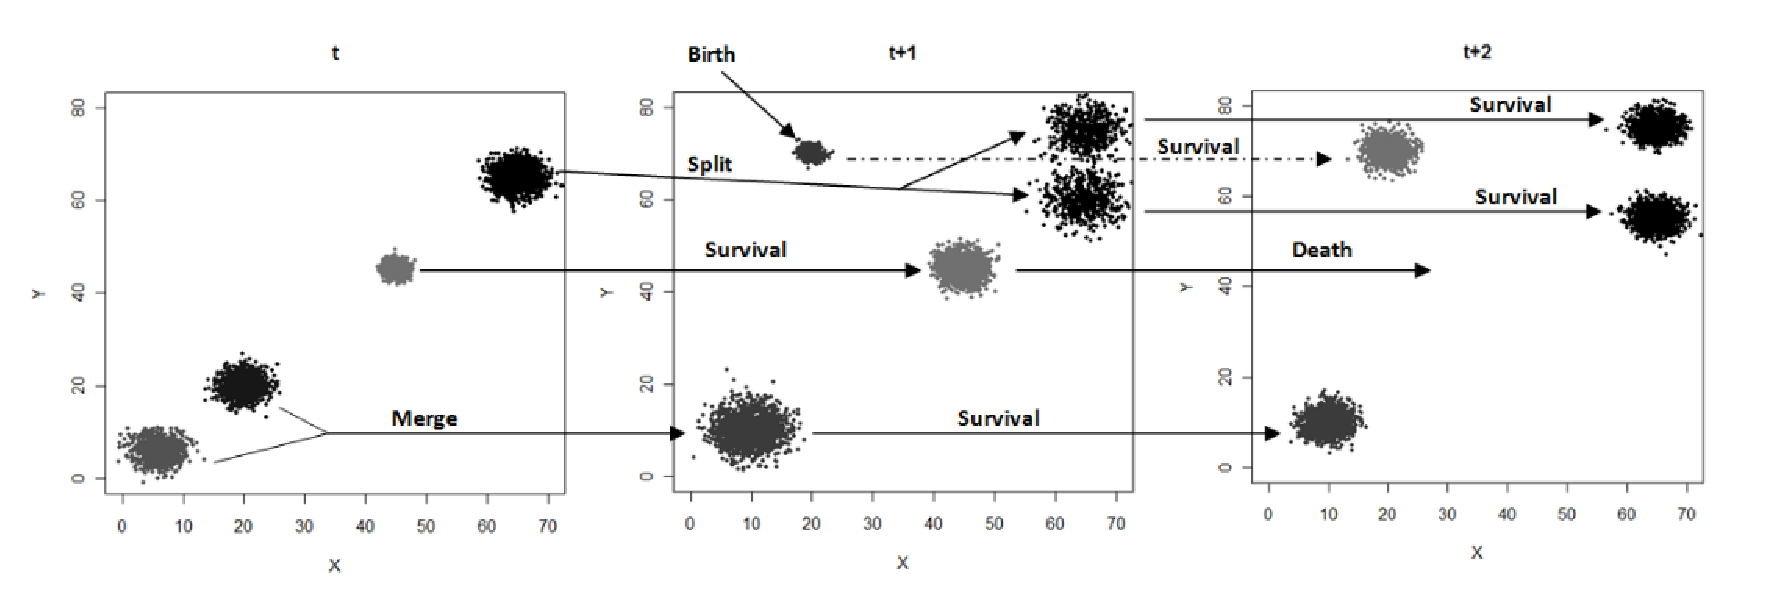
\includegraphics[height=1.15in]{evolution}
  \caption{Demonstration of five types of evolution}
\end{figure}

\subsection{Tracking and Mapping}
The central point of determinate a transaction is finding the mapping relationship between all of the points of two clusters over a specific time interval $[t_{i-\Delta t}, t_i]$. To do so, its critical to discover overlapping region with in the feature space or, in other words, the matches of clusters. In this essay the mapping relationship between two clusters are defined with a conditional probability. The clustering of two time stamps are considered as a bipartite graph. Each cluster within either time point are treated as a vertex of corresponding party of bipartite graph. The Edges of the graph connect every pair of possible connections between clusters obtained at consecutive time points. And the weight of edges are assigned by the conditional probabilities between two of them. Under this deterministic context it could describe the similarity between them thus translate the transitions into a graphical way to visualize them. If the conditional probability of two clusters outstrips a threshold, it could be convinced that those two clusters are basically the same clusters, or the later is a cluster after several translations of former one. The structure of bipartite graph is showed in Figure 2.

\begin{figure}
  \centering
  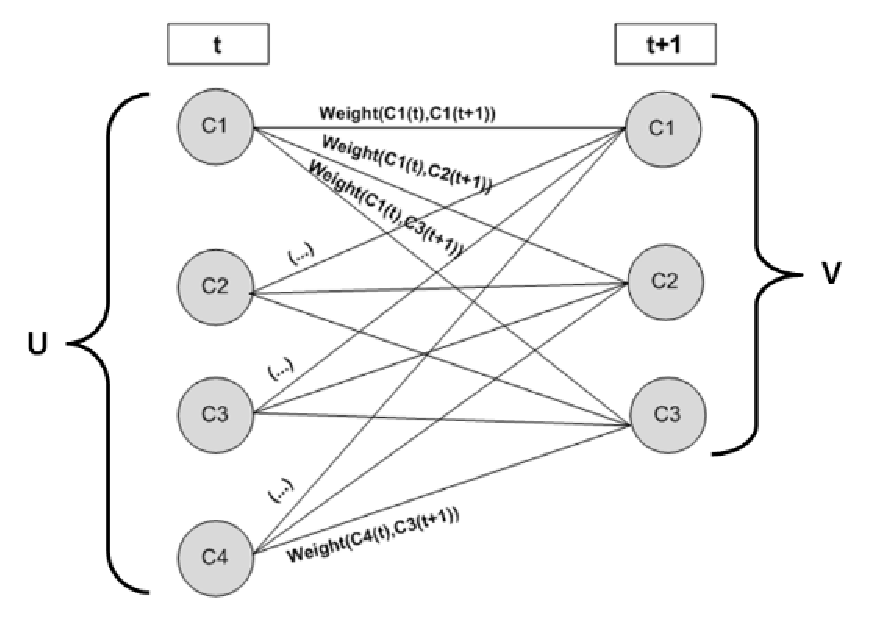
\includegraphics[height=2.3in]{biparite_graph}
  \caption{Demonstration of five types of evolution}
\end{figure}

And the formal definition of weighted bipartite graph could is such:

Given the clusterings $\upsilon_i, \upsilon_{i+\Delta t}$, a graph G=(U, V, E) can be constructed, where U represents the first subset of vertices (clusters of $t_i$), V represents the second subset of vertices (clusters of $t_{i+\Delta t}$), and E denotes a set of weighted edges between any pair of clusters belonging to $\upsilon_i$ and $\upsilon_{i+\Delta t}$. Formally, the weight assigned to the edge connecting clusters $C_m(t_i)$ and $C_u(t_{i+\Delta t})(m = (1,...k_{t_i}))$and $u = (1,...,k_{t_{t_\Delta t}})$, where $k_{t_i}$ and $k_{t_{i+\Delta t}}$ are the numbers of clusters returned by a given clustering algorithm in time points $t_i$ and $t_{i+\Delta t}$, respectively) are estimated in accordance with the conditional probability:
\begin{gather*}\
  weight(C_m(t_i), C_u(t_{i+\Delta t})) \\
   = P(X\in C_u(t_{i+\Delta t})|X\in C_m(t_i)) \\
   = \frac{\sum P(x\in C_m(t_i)\cap C_u(t_{i+\Delta t}))}{\sum P(x\in C_m(t_i))}
\end{gather*}
where X is the set of data sets contained by cluster $C_m(t_i)$ and $P(X\in C_u(t_{t+\Delta t})|X\in C_m(t_i))$ means that under the condition of given $X$ belongs to cluster $C_m(t_i)$ the probability that X is contained by $C_u$ at $t_{i+\Delta t}$.

The formula above only works under situations of crisp clustering. If we want to make it adequate to fussy clusters, some adjustment on the definition of metrics have to be done. For instance, it's mentioned in the essay that for fuzzy clustering, the $union$ of two clusters $A$ and $B$ could be defined as:
\begin{displaymath}
  A\cup B=max[A(x), B(x)]
\end{displaymath}
and analogous, the $intersection$ of them could be modified as:
\begin{displaymath}
  A\cap B=min[A(x),B(x)]
\end{displaymath}

In order to find the intersection of two clusters on different time points, each observations within the data set should be structurally identical. That is to say, we have to identify each observation on every time point and track it from it's occurrence to disappearance. Intuitively it may sound like a drawback of performance of the framework, but according to the essay this tracking of identical observations can be of major interest.

To detect different transactions between adjacent time points, the paper also introduces a threshold called \textbf{split threshold} $\lambda$ and a \textbf{survival threshold} $\tau$, which is based on the design of MONIAC's framework's external transitions\cite{SPILIOPOULOU:transition}. The mathematical description of transitions are in Table 2

\begin{table*}
  \centering
  \caption{Formal definition of the external transitions of a cluster represented by enumeration}
  \begin{tabular}{|c|c|l|}
    \hline
    \textbf{Transitions' Taxonomy}&\textbf{Notation}&\textbf{Formal Definition}\\ \hline

    Cluster's Birth & $\emptyset \rightarrow C_u(t_{i+\Delta t})$ & $0 < weight (C_m(t_i), C_u(t_{i+\Delta t}))<\tau\forall_m$ \\ \hline

    Cluster's Death & $C_m(t_i)\rightarrow\emptyset$ & $weight(C_m(t_i), C_u(t_{i+\Delta t}))<\lambda \forall_u$\\ \hline

    Cluster's Split & $C_m(t_i)\rightarrow{C_1(t_{i+\Delta t}),...C_r(t_{i+\Delta t})}\land$ & $(\exists_u\exists_v:weight(C_m(t_i), C_u(t_{i+\Delta t}))\geq\lambda\land$\\
    & $C_m(t_i)\subset{C_1(t_{i+\Delta t}),...C_r(t_{i+\Delta t})}$ & $weight(C_m(t_i), C_v(t_{i+\Delta t}))\geq\lambda)\land$\\
    &&$\sum_{u=1}^{r}weight(C_m(t_i), C_u(t_{i+\Delta t}))\geq\tau$\\ \hline

    Cluster's Merge & ${C_1(t_i),...,C_p(t_i)}\rightarrow C_u(t_{i+\Delta t})\land$ & $(weight(C_m(t_i), C_u(t_{i+\Delta t})\geq\tau)\land$\\
    & ${C_1(t_i),...,C_p(t_i)}\subset C_u(t_{i+\Delta t})$ & $\exists C_p\in\upsilon_i\setminus{C_m}:weight(C_p(t_i),C_u(t_{i+\Delta t}))\geq\tau$\\ \hline

    Cluster's Survival & $C_m(t_i)\rightarrow C_u(t_{i+\Delta t})$ & $(weight(C_m(t_i), C_u(t_{i+\Delta t}))\geq\tau)\land$\\
    &&$\nexists C_p\in\upsilon_i\setminus{C_m}:weight(C_p(t_i), C_u(t_{i+\delta t}))\geq\tau$\\ \hline
  \end{tabular}
\end{table*}

Now are some explanations to the huge table above:

A cluster is \textbf{born}, when the weight of edges which connect this cluster to each clusters of previous time point is under the survive threshold $\tau$, or, in other word, it's not possible to find a predecessor from which this cluster transforms not 'so much'.

A cluster \textbf{dies}, when the weight of all edges link from it self to a successor are under the survival threshold.

A cluster \textbf{splits} into a set of successive clusters, when at least two clusters $C_u(t_{i+_\Delta t})$ and $C_v(t_{t+\Delta t})$ exist, whose edges' weights are equal or exceed the split threshold $\lambda$ given that they are split from $C_m(t_i)$ (corresponding the conditional probability). And at the same time their sum is equal, or exceed the survival threshold.

A set of clusters \textbf{merge}, when there are at least two different clusters form $t_i$, whose connections to a given cluster of $t_{i+\Delta t}$ are equal, or exceed the survival threshold.

A cluster \textbf{survives}, when there is one and only one cluster at time point $t_{\Delta t}$, the link between whom and it has weight equal, or exceed the survival threshold.

\section{Thresholds' Sensitivity Analysis}
After defining the toxicology of transactions, we still have to face to a problem of determination of two threshold values. Thus the writer begins with a threshold's sensitivity analysis. The experiments are conducted under that all values of survival threshold within the range [0.5, 1], which is to say, if a cluster survives, there must be at least a half of observations within time point $t_i$ that maintain till the time point $t_{\Delta t}$. And for the values of the split threshold, they all fall into [0, 0.4]. The analysis is performed using \emph{ceteris paribus}.
\subsection{Survival Threshold}
Before the conduction of experiment, the writer gives a logical hypothesis that one would expect that the higher the value of the survival threshold $\tau$, the smaller the number of survival and merges detected. It wold also be expected that the increase of $\tau$ leads to a greater number of births, death and splits. Also according to the result of experiment with some value of survival threshold the transaction \emph{merge} could be replaced by \emph{survive}, since the weight assigned to one of the edges became lower than the threshold. And the number of \emph{death}s increases for higher values of the threshold.
\subsection{Split Threshold}
Logical hypothesises also can be made for split threshold $\lambda$. It's expected that the higher its value, the greater the number of deaths and \emph{birth}s, and lower the number of \emph{split}s. It could also be inferred that number of \emph{merge}s and \emph{survival}s are not affected by the variation of $\lambda$, based on the formal definition of these transitions.
\subsection{Discussion}
The thresholds' sensitivity analysis concludes that it is survival threshold that lead to completely different results, while the split threshold dosen't has a significant impact on the behavior of framework.

\section{Real World Observation Tests}
After analysing the parameters, the writer at last decides to use $\lambda=0.2$ and $\tau=0.6$ describing the method of identification of transitions, this paper also conducts several experiment with the data from real world, especially from finance territory. Data extracted from Banco de Portugal's Central Balance-Sheet Database and \emph{The data Page} of New York University - Leonard N. Stern School of Business in order to capture and understand the general trends of cluster evolution. The result does work well for the large amount of data set and perform a intuitive accuracy.

\section{Conclusion and Future Work}
In the paper a framework of monitoring evolutions of clustering structures overtime be introduced. Also the various types of transaction are categorized and the frame work is tested with real-world case using economic and financial data set. The shortage of the current framework is that it dosen't adapt to the fuzzy clustering situation and should be mended at the future.

\bibliographystyle{abbrv}
\bibliography{sigproc}
\end{document}
